\chapter{Использование симуляции для изучения системы}\label{chap:lab04}

В ходе данной лабораторной работы слушатели ознакомятся со способами изучения состояния симулируемой системы, отладки приложений, в том числе с символьной информацией, запущенных под управлением гостевой ОС.

Хотя для отладки приложений непосредственно на хозяйской системе существует достаточно широкий набор инструментов, например GDB~\cite{gdb}, WinDbg~\cite{windbg} и KВ, в ряде сценариев, таких как отладка системного кода BIOS или ОС, симуляция обеспечивает определённые удобства и преимущества, например, отсутствие необходимости использовать отдельную физическую машину для запуска отладчика. На ранних стадиях загрузки системы, когда никакой отладчик ещё не может быть подключен, моделирование является единственным решением.

Подробная информация о поддерживаемых методах отладки в Simics содержится в~\cite{analyzer, hindsight}.

\section{Цель занятия}

\begin{itemize*}
    \item Научиться подготавливать модель к символьной отладке приложений.
    \item Изучить команды инспектирования состояния гостевой системы.
\end{itemize*}

\section{Ход работы}

В приведённом ниже эксперименте мы будет изучать поведение гостевого приложения средствами инспектирования состояния и символической отладки, присутствующими в Simics. В нашем примере имя этого приложения --- \texttt{debug_example}.

\subsection{Подготовка исследуемой программы}

Исходный код программы \texttt{debug_example.c}, содержащей ошибку, находится в приложении~\ref{chap:debug-example}. Скомпилируйте \texttt{debug_example.c} для архитектуры x86, используя флаг \texttt{-m32}, и с включением отладочной информации в исполняемый файл, флаг \texttt{-g}.

\begin{lstlisting}
gcc -m32 -g -static debug_example.c -o debug_example
\end{lstlisting} 

\subsection{Подготовка гостевой системы}

\begin{enumerate}

\item Загрузите Simics со стартовым скриптом \texttt{viper-busybox.simics} в конфигурации с процессором класса \texttt{core-i7-single}:

\begin{lstlisting}
$ ./simics -e '$cpu_class=core-i7-single' targets/x86-x58-ich10/viper-busybox.simics
\end{lstlisting}

\item Включите режим обратного исполнения. Затем запустите симуляцию:
\begin{lstlisting}
simics> enable-reverse-execution
simics> continue
\end{lstlisting}

\item После того как гостевая система загрузится, авторизуйтесь и примонтируйте хозяйскую файловую систему и скопируйте файл изучаемого приложения внутрь гостя
\begin{lstlisting}
busybox login: root
~ # mount /host
~ # cp /host/home/user/debug_example ./
~ # chmod +x debug_example
\end{lstlisting}

\item Проверьте настройки отладчика запуском симуляции и командой:
\begin{lstlisting}
simics> viper.software.list
\end{lstlisting}

Вывод в консоль должен содержать список запущенных процессов на гостевой системе.
\begin{lstlisting}
Process Binary PID TID
kthreadd 2
migration/0 3
ksoftirqd/0 4
watchdog/0 5
migration/1 6
ksoftirqd/1 7
watchdog/1 8
events/0 9
events/1 10
khelper 11
async/mgr 14
sync_supers 98
bdi-default 100
kblockd/0 102
kblockd/1 103
kseriod 113
rpciod/0 132
rpciod/1 133
khungtaskd 159
kswapd0 160
aio/0 208
aio/1 209
nfsiod 217
crypto/0 223
crypto/1 224
flush-1:0 967
kjournald 957
init 1 1
sh 974 974
httpd 973 973
telnetd 971 971
\end{lstlisting}

\item Для того чтобы сконфигурировать отладчик, создайте объект символьной таблицы.
\begin{lstlisting}
simics> new-symtable debug_example
Created symbol table 'debug_example'
debug_example set for context viper.cell_context
\end{lstlisting}

\item Затем загрузите символьную информацию из исполняемого файла в созданный объект.
\begin{lstlisting}
simics> viper.software.track node = debug symtable = debug_example
Context debug0 will start tracking debug when it starts
simics> debug_example.load-symbols debug_example
\end{lstlisting}

\end{enumerate}

\subsection{Инспектирование состояния гостевой системы}

\subsubsection{Окно просмотра регистров}

Основное состояние центрального процессора хранится в его регистрах. Для просмотра регистров в Simics используется окно \textbf{CPU registers}, вызываемое через меню главного окна или через команду консоли \texttt{win-cpu-registers}. На рис.~\ref{fig:win-cpu-register-integer} и~\ref{fig:win-cpu-registers-system} показаны примеры содержимого двух вкладок этого окна. Также регистры можно просмотреть с помощью команды \texttt{pregs}:

\begin{lstlisting}
simics> pregs -all

64-bit mode
rax = 0x00007fff387d56a0             r8  = 0x000000000000000b
rcx = 0x0000000000000004             r9  = 0x000000000000000f
rdx = 0x00007fff387d5758             r10 = 0x000000000000000b
rbx = 0x0000000000400e30             r11 = 0x0000000000000008
rsp = 0x00007fff387d5660             r12 = 0x0000000000000000
rbp = 0x00007fff387d5670             r13 = 0x0000000000000000
rsi = 0x00007fff387d5748             r14 = 0x0000000000000000
rdi = 0x0000000000000001             r15 = 0x0000000000000000

rip = 0x00000000004004c3, linear = 0x00000000004004c3

eflags = 0 0 0 0 0 0 0 0 0 0 0 0 1 0 0 0 0 0 0 1 1 0 = 0x00000206
         I V V A V R - N I I O D I T S Z - A - P - C
         D I I C M F   T O O F F F F F F   F   F   F
           P F           P P                        
                         L L                        

es   = 0x0000, base = 0x00000000, limit = 0x0, attr = 0x0
cs   = 0x0033, base = 0x00000000, limit = 0xffffffff, attr = 0xa0fb
ss   = 0x002b, base = 0x00000000, limit = 0xffffffff, attr = 0xc0f3
ds   = 0x0000, base = 0x00000000, limit = 0x0, attr = 0x0
fs   = 0x0063, base = 0x02024860, limit = 0xffffffff, attr = 0xc0f3
gs   = 0x0000, base = 0x00000000, limit = 0x0, attr = 0x0
tr   = 0x0040, base = 0xffff88007fc0f900, limit = 0x2087, attr = 0x8b
ldtr   = 0x0000, base = 0x00000000, limit = 0xffff, attr = 0x82
idtr: base = 0xffffffff81b85000, limit = 00fff
gdtr: base = 0xffff88007fc04000, limit = 0007f

efer = 1 1 - 1 -- 1 = 0x00000d01
       N L   L    S
       X M   M    C
       E A   E    E

cr0 = 1 0 0 -- 1 - 1 -- 1 1 0 0 1 1 = 0x80050033
      P C N    A   W    N E T E M P
      G D W    M   P    E T S M P E

cr2 = 0x000000000040c930
cr3 = 0x000000007c01b000

cr4 = 0 - 1 1 0 1 1 1 1 0 0 0 0 = 0x000006f0
      V   O O P P M P P D T P V
      M   S S C G C A S E S V M
      X   X F E E E E E   D I E
      E   M X
          M S
          E R
          X
          C
          P
          T

dr0 = 0x0000000000000000 disabled
dr1 = 0x0000000000000000 disabled
dr2 = 0x0000000000000000 disabled
dr3 = 0x0000000000000000 disabled

dr6 = 0 0 0 -- 0 0 0 0 = 0xffff0ff0
      B B B    B B B B
      T S D    3 2 1 0

dr7 = 00000400

<Вывод опущен>
\end{lstlisting}

\begin{figure}[htb]
    \centering
    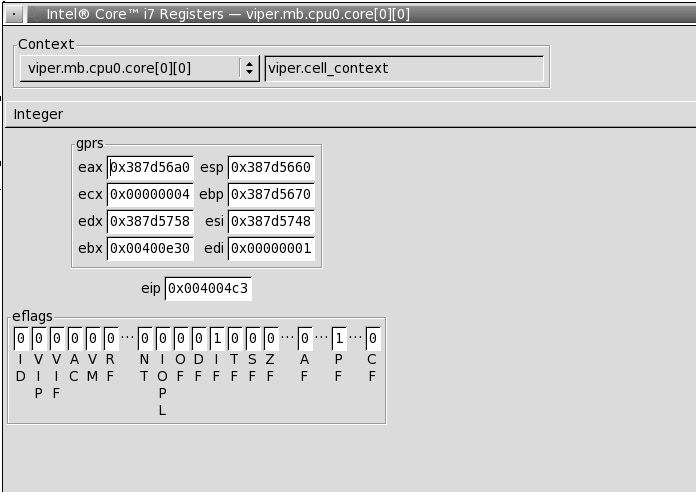
\includegraphics[width=0.6\textwidth]{./images/win-cpu-registers-integer.png}
    % win-cpu-registers-integer.png: 696x492 pixel, 96dpi, 18.41x13.02 cm, bb=0 0 522 369
    \caption{Окно просмотра регистров. Вкладка с регистрами общего назначения}
    \label{fig:win-cpu-register-integer}
\end{figure}

\begin{figure}[htb]
    \centering
    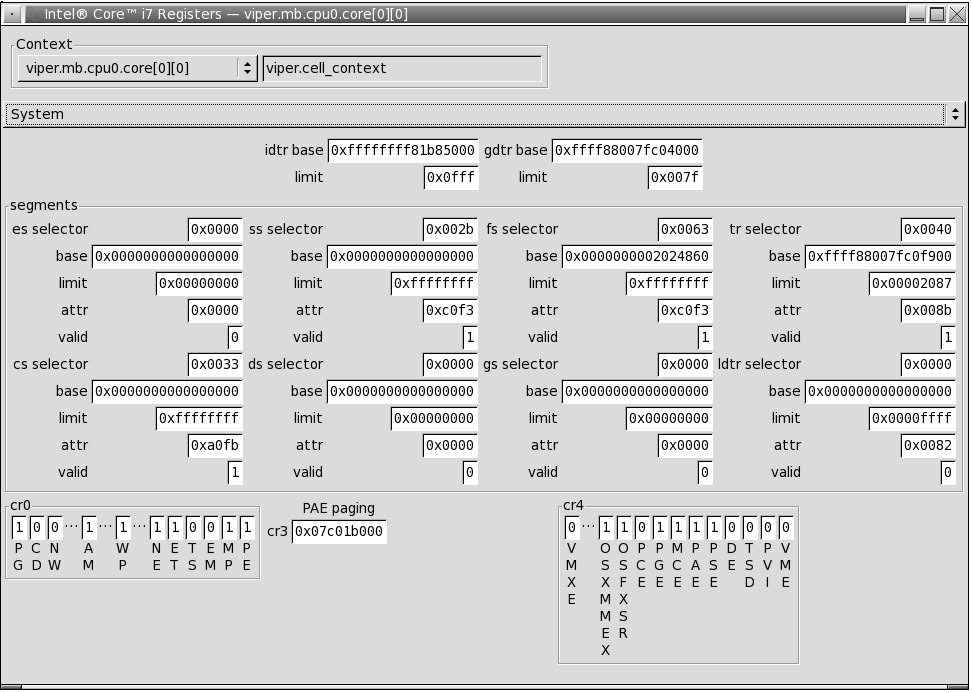
\includegraphics[width=0.8\textwidth]{./images/win-cpu-registers-system.png}
    % win-cpu-registers-system.png: 972x693 pixel, 96dpi, 25.71x18.33 cm, bb=0 0 729 520
    \caption{Окно просмотра регистров. Вкладка с системными регистрами}
    \label{fig:win-cpu-registers-system}
\end{figure}

\subsubsection{Память системы}

Для просмотра различных пространств памяти, присутствующих в моделируемой системе, используется окно \textbf{Memory Contents}, вызываемое также командой \texttt{win-memory} (рис.~\ref{fig:win-memory}).

\begin{figure}[htb]
    \centering
    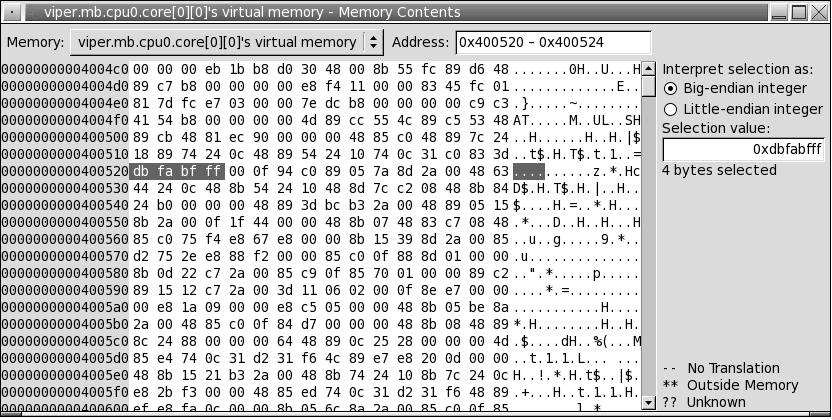
\includegraphics[width=0.8\textwidth]{./images/win-memory.png}
    % win-memory.png: 832x420 pixel, 96dpi, 22.01x11.11 cm, bb=0 0 624 315
    \caption{Окно просмотра содержимого памяти системы}
    \label{fig:win-memory}
\end{figure}

\subsection{Начало отладки}

Поставьте точку останова на функции \texttt{main()} и запустите симуляцию.
\begin{lstlisting}
simics> break (pos main) -x
Breakpoint 92 set on address 0x80485c6 in 'viper.cell_context' with access mode 'x'
simics> continue
\end{lstlisting}

В гостевой ОС запустите исполняемый файл \texttt{debug_example}. Симуляция должна остановиться с выводом в консоль:
\begin{lstlisting}
Breakpoint 922 on instruction fetch from 0x80485c6 in viper.cell_context.
[viper.mb.cpu0.core[0][1]] cs:0x00000000080485c6 p:0x07c17e5c6  lea ecx,4[esp]
Setting new inspection cpu: viper.mb.cpu0.core[0][1]
main (argc=, argv=) at /nfs/ims/home/mvchurik/working_folder/debug_example.c:53
53      (file /nfs/ims/home/mvchurik/working_folder/debug_example.c not found)
\end{lstlisting}

% Перейдите к окну отладки.
\begin{lstlisting}
simics> win-source-view
\end{lstlisting}
Убедитесь, что поле \textbf{Source File}  окна \textbf{Source Code} (рис.~\ref{fig:win-source-view}) заполнено. В противном случае загрузите в окно исходный файл кнопкой \textbf{Find}.

\begin{figure}[htb]
    \centering
    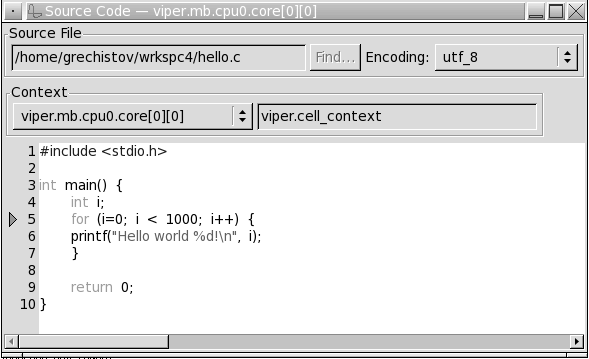
\includegraphics[width=0.6\textwidth]{./win-source-view.png}
    \caption{Окно просмотра исходного кода}
    \label{fig:win-source-view}
\end{figure}

\subsection{Окна с информацией для символической отладки}

Так как мы предварительно загрузили символьную информацию о приложении, то для его символьной отладки могут быть использованы дополнительные окна, такие как окно исходного кода (рис.~\ref{fig:win-source-view}), дизассемблера (рис.~\ref{fig:win-disassembly}) и стека (рис.~\ref{fig:win-stack-trace}). Информация, содержащаяся в них, также может быть получена с помощью команд \texttt{list <имя функции>}, \texttt{disassemble <адрес> <количество>} и \texttt{stack-trace}.

\begin{figure}[htb]
    \centering
    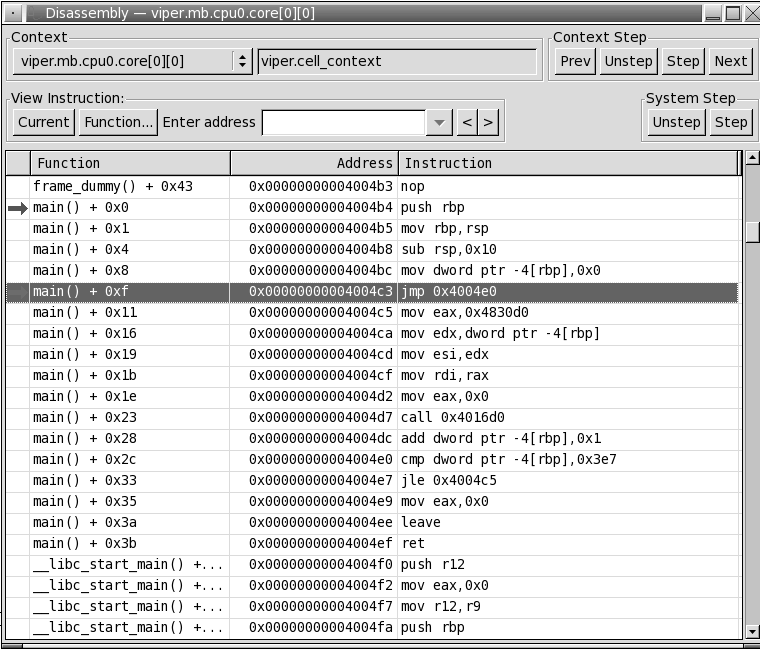
\includegraphics[width=0.6\textwidth]{./images/win-disassembly.png}
    \caption{Окно дизассемблера}
    \label{fig:win-disassembly}
\end{figure}

\begin{figure}[htb]
    \centering
    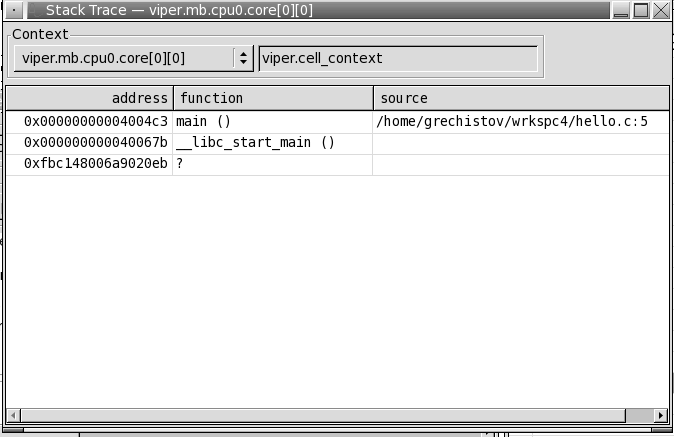
\includegraphics[width=0.6\textwidth]{./images/win-stack-trace.png}
    % win-stack-trace.png: 674x437 pixel, 96dpi, 17.83x11.56 cm, bb=0 0 505 328
    \caption{Окно просмотра стека}
    \label{fig:win-stack-trace}
\end{figure}


\subsection{Управление исполнением программы}

Теперь, когда симуляция находится внутри интересующей нас программы, отладчик должен позволять инспектировать состояние её переменных, положение указателя текущей инструкции, а также управлять пошаговым исполнением её операций. Для нас окажутся полезными следующие команды Simics.

\begin{enumerate*}
    \item \texttt{sym} --- получить значение переменной, определённой в текущем контексте гостевой программы.
\begin{lstlisting}
simics> sym argc
1
\end{lstlisting}

\item \texttt{step-line} --- выполнить одну строку исходного кода отлаживаемой программы и остановиться.
\item \texttt{next-line} --- выполнить одну строку исходного кода отлаживаемой программы и остановиться, при этом пропустив выполнение подпроцедур, если они вызываются.
\item \texttt{pos} --- узнать адрес функции или строки кода:
\begin{lstlisting}
simics> pos main
0x804832e
simics> pos debug_example.c:5
0x8048260
\end{lstlisting}

\end{enumerate*}

Кроме задания этих команд, управление исполнением может осуществляться с помощью кнопок \textbf{Step} и \textbf{Next} окна Disassembly (рис.~\ref{fig:win-disassembly}).

\subsubsection{Использование точек останова}

\paragraph{Доступы в память.}

Самый простой и часто используемый тип --- это точка останова по виртуальному адресу исполняемой инструкции:

\begin{lstlisting}
simics> break 0x4004b4
Breakpoint 1 set on address 0x4004b4 in 'viper.cell_context' with access mode 'x'
\end{lstlisting}

Кроме инструкций, точки останова могут быть созданы для регионов данных, при этом попытка гостевой программы обратиться к такому региону вызовет остановку симуляции. Формат команды при этом включает дополнительные флаги \texttt{-r} и \texttt{-w} для указания, должна ли она реагировать на чтение или запись памяти:

\begin{lstlisting}
simics> break 0x7fffdc2b3d7c -r -w
Breakpoint 2 set on address 0x7fffdc2b3d7c  in 'viper.cell_context' with access mode 'rw'
\end{lstlisting}

Полный формат команды \texttt{break} позволяет выбрать любую комбинацию флагов, а также указать длину наблюдаемого диапазона в байтах:
\begin{lstlisting}
break <address> [length] [-r] [-w] [-x]
\end{lstlisting}

Для того чтобы увидеть данные обо всех установленных точках останова, используется команда \texttt{list-breakpoints}.

\paragraph{Исключения.}

Другой класс событий, который может наблюдаться в отладчике, --- это архитектурные исключения. Для установки таких точек используется команда:

\begin{lstlisting}
break-exception name = Page_Fault_Exception
\end{lstlisting}

Полный список допустимых событий достаточно длинен; нас будут интересовать следующие из них: \texttt{Page_Fault_Exception}, \texttt{General_Protection_Exception}, \texttt{Invalid_Opcode_Exception}.

Точка останова прерывает исполнение симуляции. Если вместо этого желательно просто наблюдать за происходящими событиями, то следует использовать команду \texttt{trace-exception}, синтаксис который аналогичен \texttt{break-exception}.

\section{Задания}

\begin{enumerate*}

    \item Начать симуляцию и передать исследуемую программу в гостевую систему.
    \item Охарактеризовать тип проблемы, возникающий при работе программы.
    \item Отладить программу с помощью Simics.
\end{enumerate*}

\section{Вопросы для самостоятельного изучения}

\begin{enumerate*}
\item Для того чтобы любой отладчик, в том числе вcтроенный в Simics, мог иметь информацию об исходном коде исследуемой программы, информация о нём должна быть доступна ему на этапе отладки. В свою очередь программа должна быть скомпилирована с  использованием особенных флагов компиляции. Выясните, какие опции должны быть использованы в случае использования компилятора GCC.

\item Для того чтобы программа, скомпилированная на хозяйской системе, могла быть успешно запущена внутри гостя, требуется соблюсти несколько условий. Одно из них --- использование т.н. статической линковки, в случае GCC обозначаемой флагом \mbox{\texttt{-static}}. Выясните, зачем был использован этот флаг. При каких условиях на гостевую и хозяйскую системы можно использовать динамическую линковку?

\end{enumerate*}

\iftoggle{webpaper}{
    \printbibliography[title={Список литературы к занятию}]
}{}